\chapter{Robotic Middleware}

In addition to computer science and engineering, the field of robotics is encompasses mechanical engineering, electrical engineering and systems engineering. Due to the complexity of robotic systems, software engineering best practices encourage us to develop abstraction layers. This allows us to re-use code and minimize the scope of each component that we develop. We will compare several robotic middleware solutions below.

Among the popular robotic middleware technologies there are a few common traits: transportation encapsulation, stream processing, remote method invocation (RPC), and configuration management.

% Do I need a section on Player?
\section{Player Framework}
An application using the Player framework is split into two parts: a client and a server. The client and server communicate over a TCP socket using the Player protocol. All communication between the client and server happens using ``interfaces''. The client can connect to a Player server, request a list of exposed interfaces, and connect up instances of those interfaces. The player server runs in a single process and dynamically loads implementations of interfaces, known as drivers, on demand at runtime. A simple Player application can be seen in Figure~\ref{fig:middleware-player}. 

\begin{figure}[ht]
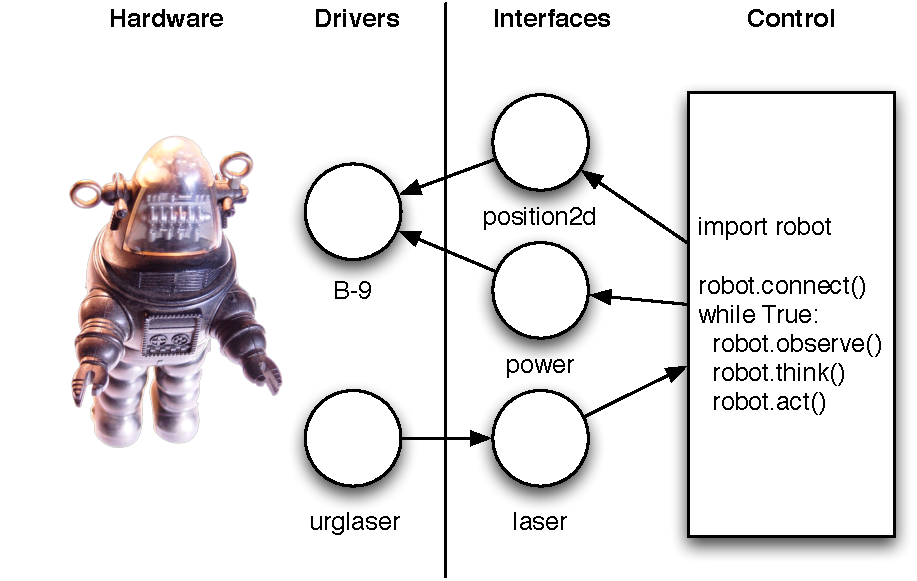
\includegraphics{images/middleware-player.pdf}
\caption{Example Player application\label{fig:middleware-player}}
\end{figure}

The Player server and drivers are written in C, however there are several language bindings for the client including C, C++ and Python. The Player server is configured at runtime using a configuration file instructing the server which drivers to load and any configuration values.

\section{Robot Operating System}
The Robot Operating System (ROS) developed by Stanford University and Willow Garage can be thought of as a child of the Common Object Request Broker Architecture (CORBA) design pattern and the Player framework. This design decision gives ROS a modern distributed architecture that encourages small, reusable code. In addition, ROS has extensive development tools and an active community base.

The ROS architecture can be thought of as a directed graph. Software components are called ``nodes'' and are run in separate processes. This allows each node to be written using the most appropriate language to the task. As an example, a performance sensitive node could be written in C while a less demanding node could be written in Python for improved readability. At the time of writing ROS supports C++, Python, Java and Lisp.

% Nodes => Package
% Pacakages => Stack
% Stack => Repositories

\subsection{Topics and Services}
ROS provides a framework for connecting nodes together. Nodes can be connected together through a ``topic'' or through a ``service''. A topic is a named stream that supports multiple readers and writers. Nodes that write to a topic are known as ``publishers''. A publisher announces that it is publishing to one or more topics to the ``roscore'' node. 

The ``roscore'' node is a special node that is run when the ROS environment is initialized. It acts as a directory server maintaining a list of active nodes, topic, services, and configuration values.

Nodes that wish to read from a topic are known as ``subscribers''. Similar to publishers, a subscriber will announce it is listening to one ore more topics to the roscore node.

The roscore node continually informs subscribers of the location of publishers. This allows nodes to communicate directly without needing to contact the roscore node. Currently only TCP and UDP unicast sockets are supported, however future releases of ROS will include shared memory and multicast networking. A simple example of a ROS digraph can be seen in Figure~\ref{fig:middleware-ros}.

\begin{figure}[ht]
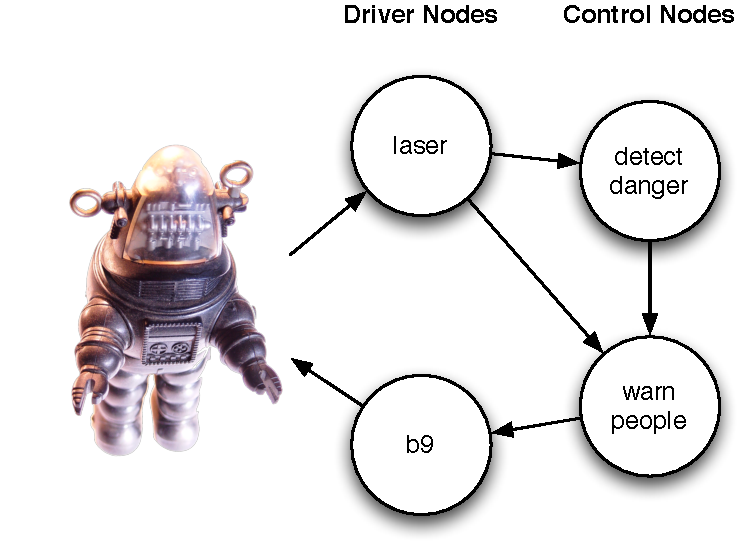
\includegraphics{images/middleware-ros.pdf}
\caption{Example ROS application\label{fig:middleware-ros}}
\end{figure}

The development of nodes can build on eachother. Low-level hardware interface nodes, akin to drivers in player, communicate raw sensor and actuator messages. Unlike Player's control code, ROS allows the developer to break the control code up into several pieces. This modular interface allows code re-use of control code as well as driver code.

% TODO: correct acronym IDL
ROS also defines a common message format for communicating. Messages are defined using a independent-domain language (IDL) which in turn auto-generate serialization and deserialization code for supported languages. An example message file can be seen in Figure~\ref{fig:point}.

\begin{figure}[ht]
\makebox[\textwidth]{\hrulefill}
\begin{verbatim}
	# This contains the position of a point in free space
	float64 x
	float64 y
	float64 z
\end{verbatim}
\makebox[\textwidth]{\hrulefill}
\caption{Point.msg : Message representation of a 3D Point\label{fig:point}}
\end{figure}

\subsection{Kinematic Tree}
A large part of the complexity of robotic systems is transforming coordinate frame in a timely manner. ROS offers a special topic located at \verb!tf! and provides a cross-language library, also called ``tf'', to ease coordinate transformation tasks.

ROS builds a kinematic tree using data published to the \verb!tf! topic. Coordinate frames contain a timestamp, an object's name, the parent coordinate frame and the quaternion offset between the two. The tf package allows a developer to request a quaternion offset between two coordinate frames. 

In order to maintain a correct representation, the library automatically discards stale coordinate frame data. This requires objects to publish their location at a specified frequency. When all nodes are publish at an acceptable rate the full kinematic tree is accessible. A sample kinematic tree for a robot with a stero-vision rig mounted on-top of a pan-tilt unit can be seen in Figure~\ref{fig:tf-example}.

\begin{figure}[ht]
\begin{center}
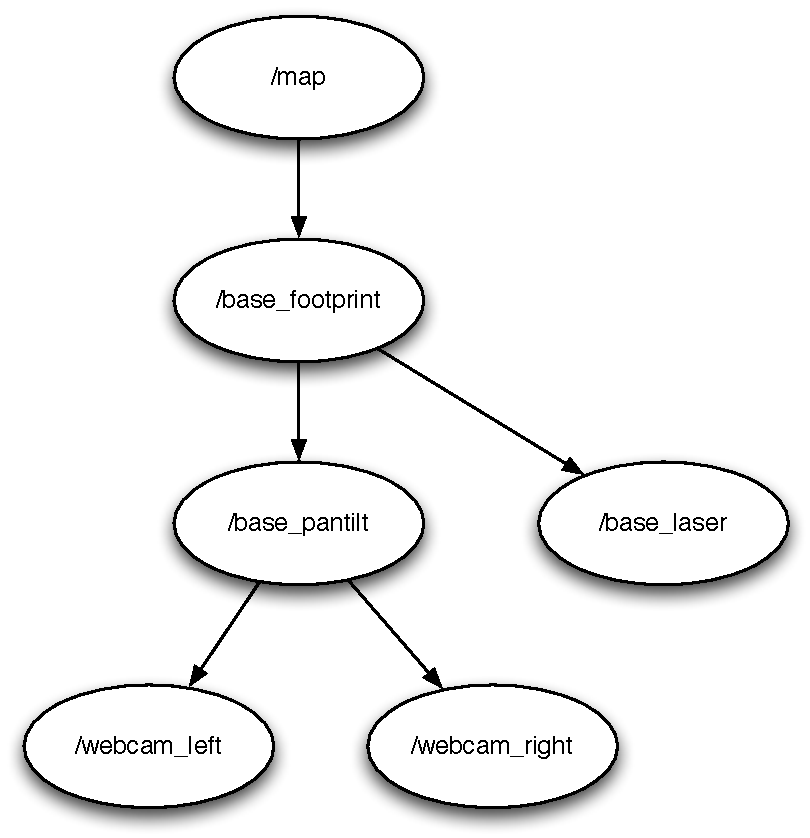
\includegraphics[width=3.5in]{images/tf-example.pdf}
\caption{Sample Kinematic Tree\label{fig:tf-example}}
\end{center}
\end{figure}

\section{RIDE Architecture}

ROS was originally designed for a single robot system. A node may only be attached to a single ROS graph (or ``realm''). RIDE is designed to work with large numbers of robots. Early on in the development cycle, I decided to stick to the model that realms are local to a robot. This allows robots to operate independently of connectivity to eachother, and does not require any changes to existing single-robot code bases. This design conflict required the development of a new node library called ``rosmultimaster''.

rosmultimaster allows a single node to connect to multiple realms using the native ROS python (rospy) codebase. rosmultimaster is multi-threaded library that provides both a synchronous and asynchronous interface. Further implementation details for rosmultimaster can be found in Appendix X % TODO: Appendix number

Using the rosmultimaster code-base, we developed RIDE to connect to each robot on startup, as well as a single mapping realm. A high level overview can be found in Figure X.X. The map realm acts as a central location to for map retrieval / updating. In the future, if ROS were to support peer-to-peer networking, a map could be dynamically built by stitching together several independent maps. 

% TODO: Generate high level figure

\subsection{Simulation Realm}
I used a simulation environment, called ``rosstage'', to provide a consistent environment. The simulated system architecture is a superset of the regular RIDE architecture with the map realm acting as a full simulation realm and several additional topics being shared to the robot realms. An overview of the simulation architecture can be found in Figure~\ref{fig:ride-simulation-realm}.

\begin{figure}[ht]
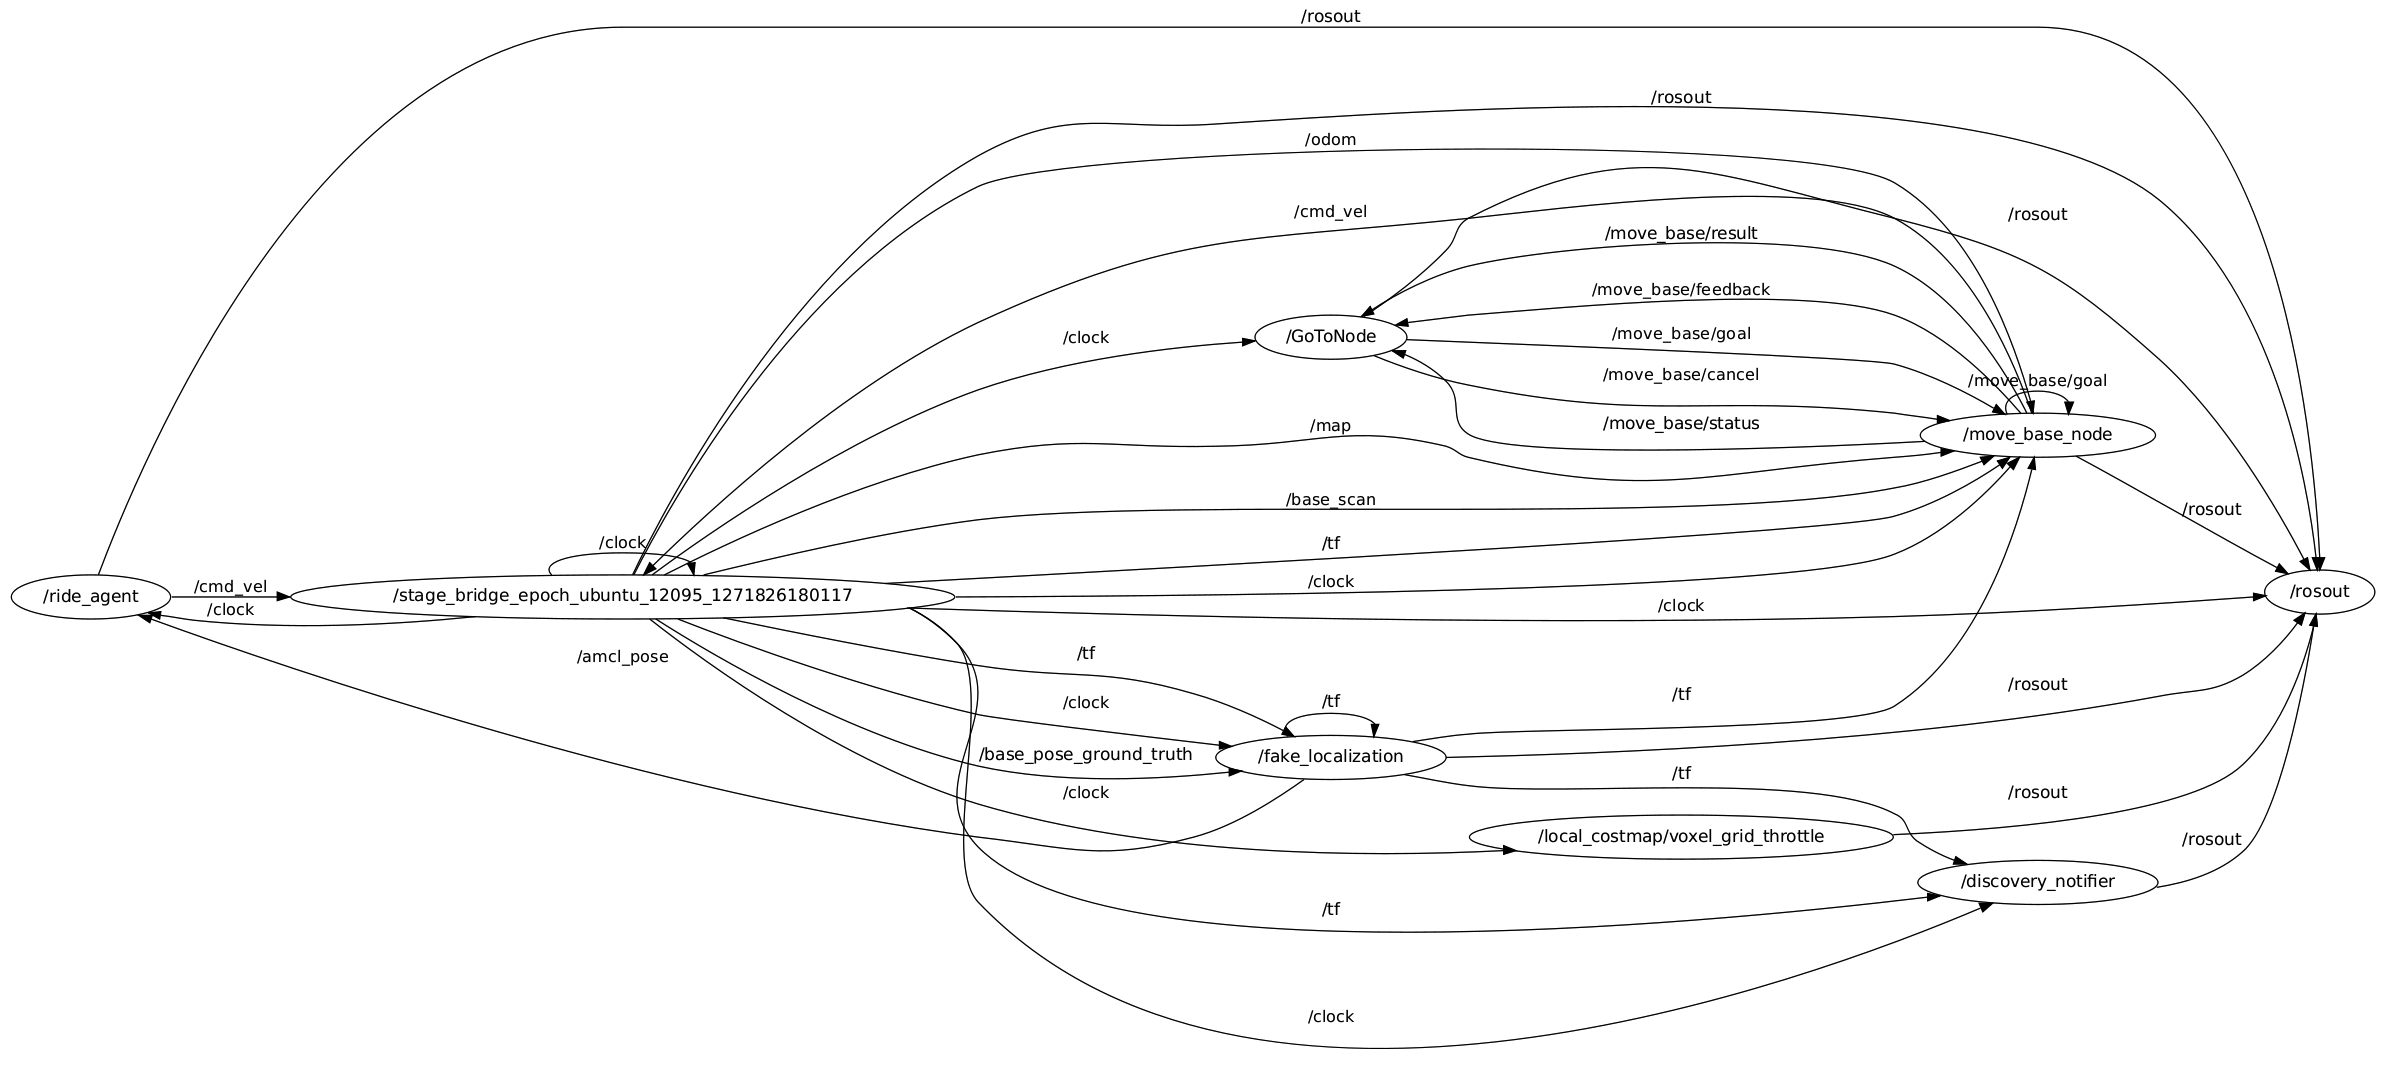
\includegraphics[width=\textwidth]{images/ride-simulation-realm.png}
\caption{Publish/Subscriber graph in RIDE Simulation Realm\label{fig:ride-simulation-realm}}
\end{figure}

\subsection{Robot Realm}
\label{section:robot-architecture}
RIDE uses a modular structure for controlling robots. Due to the topic system in ROS, this functionality can be written to work regardless of if the robot is simulated or physical. Each robot must provide position data for basic RIDE functionality. Beyond position data, the user can choose what sensors, actuators, and ``actions'' to provide.

Figure~\ref{fig:ride-robot-realm} demonstrates a simulated robot realm and the components to the most basic functionality. The robot must be able to orient itself with respect to the \verb!/map! coordinate frame. This typically requires a localization node like the Adaptive Monte-Carlo Localization (amcl) node when running on a physical robot or a fake localization node when running in simulation.

In addition to providing position data, the robot must expose a path planning node. ROS provides a navigation stack complete with a path planning node, called move\_base. Lastly, the robot must provide a way to directly control the movement of the robot allowing the user to ``drive'' a robot around freely.

\begin{figure}[ht]
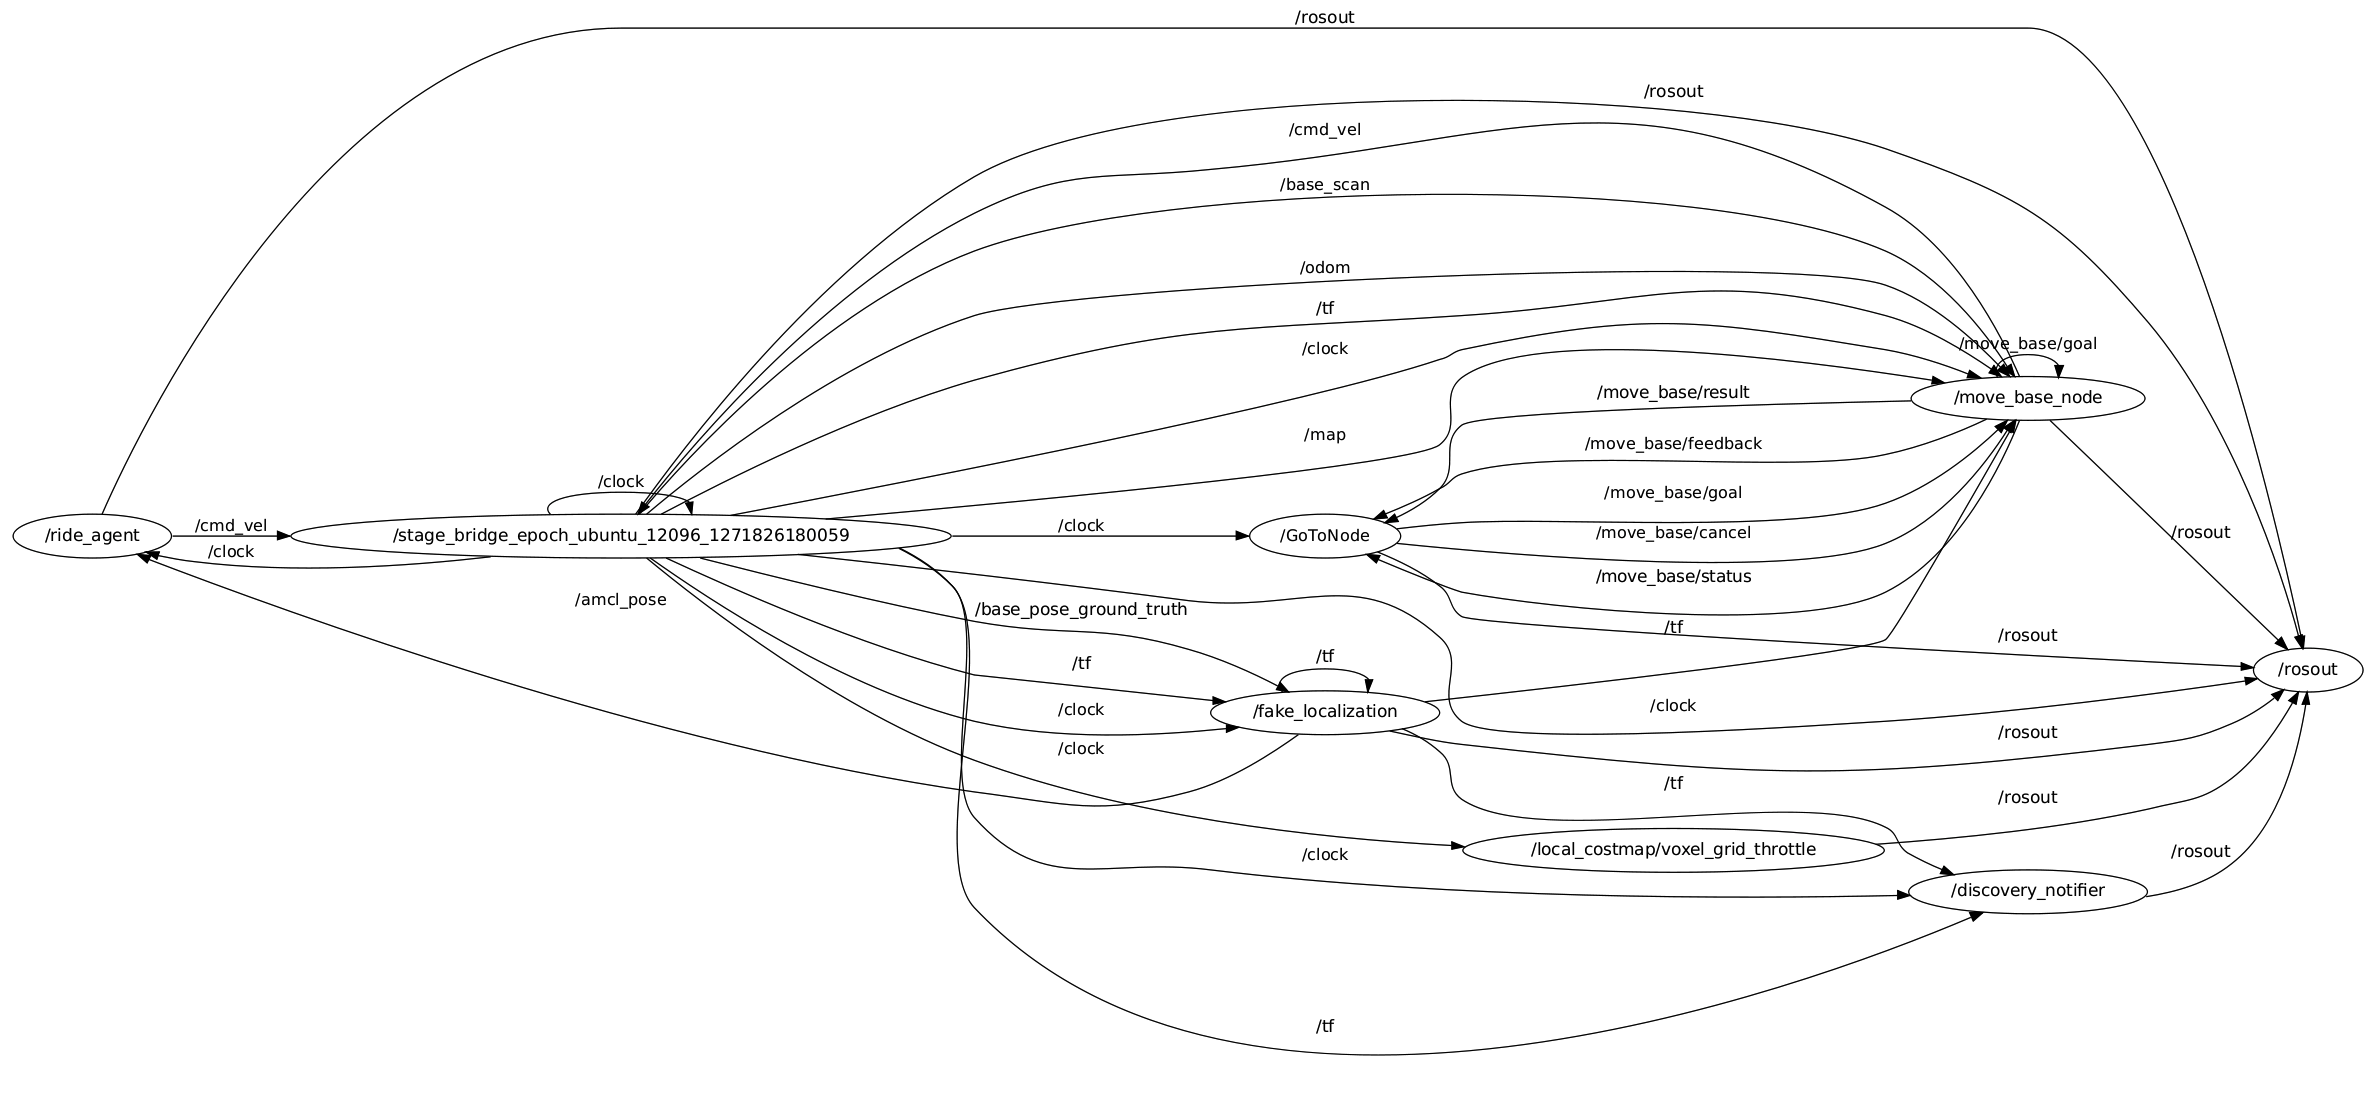
\includegraphics[width=\textwidth]{images/ride-robot-realm.png}
\caption{Publish/Subscriber graph in RIDE Robot Realm\label{fig:ride-robot-realm}}
\end{figure}

% Discuss ride_agent
% Discuss GoToNode

\section{Panda3D Integration}

RIDE uses the popular 3D rendering engine Panda3D to display the virtual environment to the user. Panda3D is implemented in C++ for performance reasons, and provides a Python interface that we used to integrate with ROS. 

Like most rendering engines, Panda3D relies on a scene graph for rendering objects onto the screen. We kept a one-to-one mapping of objects in ROS's kinematic tree to objects in Panda3D's scene graph. This natural mapping proved to be simple and effective.

We developed a simple configuration file, using the YAML format, to let users configure which realms RIDE should connect to and what models to use when rendering objects from ROS's kinematic tree in the Panda3D scene graph. An example can be seen Figure X.X, where a single robot contains a laser range finder. Future work would remove the configuration file, moving the connection information into the user interface, and updating the RIDE protocol to provide dimensions and model information as needed.

% TODO: Insert figure: RRS / scene graph

Panda3D provides its own run loop for running tasks, processing events and updating the scene graph. For performance reasons, Panda3D does not use the native Python threading implementation so I chose to use the synchronous API offered by rosmultimaster. I then added one background task per rosmultimaster instance to Panda3D's task manager. The rosmultimaster tasks were called at a specified frequency designed to keep latency low and framerate high.
